% !TeX root = RJwrapper.tex
\title{\pkg{miWQS}: Multiple Imputation Using Weighted Quantile Sum Regression}
\author{by Paul M. Hargarten and David C. Wheeler}

\maketitle

\abstract{%
The \pkg{miWQS} package in the Comprehensive R Archive Network (CRAN)
utilizes weighted quantile sum regression (WQS) in the multiple
imputation (MI) framework. The data analyzed is a set/mixture of
continuous and correlated components/chemicals that are reasonable to
combine in an index and share a common outcome. These components are
also interval-censored between zero and upper thresholds, or detection
limits, which may differ among the components. This type of data is
found in areas such as chemical epidemiological studies, sociology, and
genomics. The \pkg{miWQS} package can be run using complete or
incomplete data, which may be placed in the first quantile, or imputed
using bootstrap or Bayesian approach. This article provides a stepwise
and hands-on approach to handle uncertainty due to values below the
detection limit in correlated component mixture problems.
}

\hypertarget{introduction}{%
\section{Introduction}\label{introduction}}

When studying public health, researchers want to determine if a
set/mixture of continuous and correlated components/chemicals is
associated with an outcome and if so, which components are important in
that mixture \citep{braunWhatCanEpidemiological2016}. These components
share a common univariate outcome but are interval-censored between zero
and low thresholds, or detection limits, that may be different across
the components.

We have created the \CRANpkg{miWQS} package to analyze epidemiological
studies with chemical exposures, but researchers may also apply the
package to public health, genomics, or other areas in public health and
medicine. Epidemiologists examine chemical mixtures because human
exposure to a large number of chemicals may increase the risk of disease
\citep{braunWhatCanEpidemiological2016}. Researchers may also create a
socioeconomic status (SES) index that is generally composed of
continuous correlated variables in the following domains: educational
achievement, race, income, housing, and employment
\citep{wheelerEstimatingAreaLevelSocioeconomic2017, wheelerExplainingVariationElevated2019}.
For example, race may be represented by percent of the population that
is white. There are several examples of this in the literature
\citep{wheelerBayesianDeprivationIndex2019, wheelerNeighborhoodDisadvantageTobacco2020}.
Although these variables may have missing values throughout the
distribution, researchers may use the \pkg{miWQS} package to create SES
index even in the presence of missing data. Alternatively, genome-wide
association studies (GWAS's) analyze DNA sequence variation using single
nucleotide polymorphisms (SNPs) \citep{bushChapter11GenomeWide2012}. As
SNPs constitute high-frequency changes of a single base in the DNA
sequence throughout the genome, SNPs serve as markers of a genomic
region \citep{bushChapter11GenomeWide2012}. Thus, SNPs are highly
correlated
\citep{bushChapter11GenomeWide2012, ferberModelingDiscreteSurvival2015}.
The research aim of a GWAS is to find associations between genes and
common and complex diseases like schizophrenia and to identify specific
associated genes. The \pkg{miWQS} package can answer this research aim
while simultaneously accounting for the correlation between SNPs.

In the data, an approach to account for the correlation among completely
observed components is the weighted quantile sum (WQS) regression
\citep{carricoCharacterizationWeightedQuantile2014, czarnotaAssessmentWeightedQuantile2015, genningsCohortStudyEvaluation2013}.
The application of WQS regression to censored data has been limited
statistically and computationally on CRAN (the Comprehensive R Archive
Network)
\citep{czarnotaAnalysisEnvironmentalChemical2015, hortonCOOccurringExposurePerchlorate2015, czarnotaWqsWeightedQuantile2015, renzettiGWQSGeneralizedWeighted2020a}.
In order to fully account for the uncertainty due to censoring, the
\pkg{miWQS} package utilizes WQS regression in the multiple imputation
(MI) framework
\citep{ hargartenAccountingUncertaintyDue2020, hargartenMiWQSMultipleImputation2021}.

As compared to other WQS packages in R, the \pkg{miWQS} package is
specifically designed to use highly correlated data that include
interval-censoring. The \CRANpkg{wqs}
\citep{czarnotaWqsWeightedQuantile2015} package performs WQS regression
only on complete mixtures that share a continuous or binary outcome. The
\code{wqs.est()} function in the \pkg{wqs} package can be used for
continuous outcomes and displays an error if fed incomplete information.
The \code{gwqs()} function in the \CRANpkg{gWQS} package runs WQS
regression when the outcome is continuous, binary, binomial,
multinomial, or a count. If incomplete components are inputted into
\code{gwqs()}, the function uses non-missing data without warning
\citep{renzettiGWQSGeneralizedWeighted2020a}. By contrast, the
\pkg{miWQS} functions are constructed to handle both complete and
incomplete mixture data that share a continuous, binary, or count
outcome by using MI.

\begin{figure}[h]

{\centering 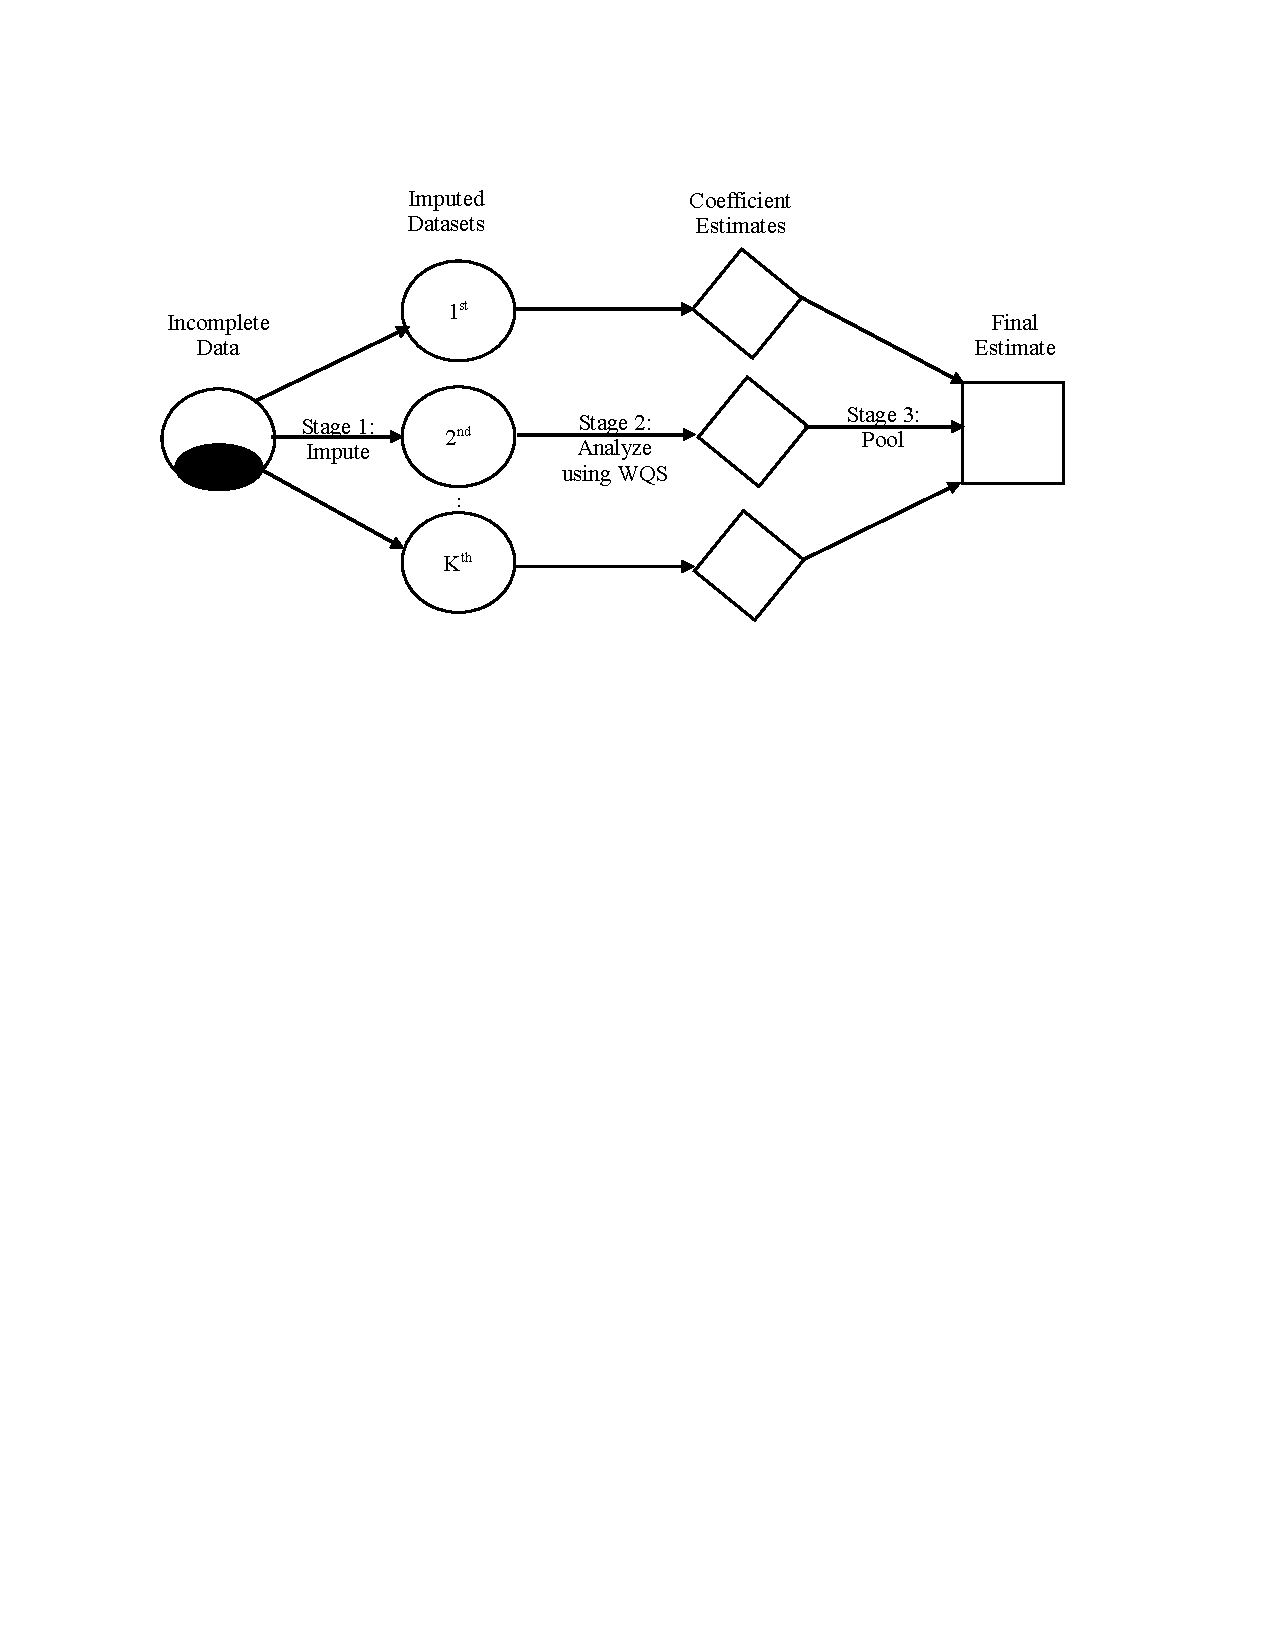
\includegraphics[width=1\linewidth]{figure-word/fig_mi_intro.pdf} 

}

\caption{\label{fig::mi} Multiple Imputation in connection with the Weighted Quantile Sum regression (MI-WQS). Given partially observed correlated chemical exposures that share a common outcome and covariates, (stage 1) researchers impute the below detection limit values (dark circles) K times to form complete datasets. In stage 2, each imputed dataset is analyzed using WQS regression. In stage 3, the coefficient estimates from the K WQS regressions (diamonds) are combined into a final estimate (square).}\label{fig:fig.mi}
\end{figure}

The MI approach provides valid statistical inference in estimating
regression parameters when data are missing
\citep{dongPrincipledMissingData2013, rubinMultipleImputationNonresponse1987, whiteMultipleImputationUsing2011}.
Specifically, MI consists of three stages: (1) imputation, (2) analysis,
and (3) pooling (Figure \ref{fig::mi}). First, we create several imputed
datasets by replacing the below the detection limit (BDL) values by
plausible data values. The complete datasets are identical for the
observed data but are different in the imputed values. Second, we
analyze each complete dataset using WQS regression to obtain estimates
\citep{carricoCharacterizationWeightedQuantile2014, czarnotaAssessmentWeightedQuantile2015, genningsCohortStudyEvaluation2013, hargartenAccountingUncertaintyDue2020}.
Lastly, we combine each WQS estimate from different analyses to form one
final estimate, to find its variance, and to perform statistical tests
in order to determine the significance of the exposure effects.

Other MI packages in R have functions that combine estimates, but these
are different than the \code{pool.mi()} function used in the \pkg{miWQS}
package. The \CRANpkg{mice} (multiple imputation by chained equations)
package implements a strategy to impute multivariate missing data using
fully conditional densities
\citep{vanbuurenMiceMultivariateImputation2011}. Its pool function
combines one estimate at a time, while \code{pool.mi()} combines all
estimates simultaneously. The \CRANpkg{norm} package allows users to
impute values with an assumed multivariate normal distribution
\citep{novoNormAnalysisMultivariate2013}. Its pool function,
\code{mi.inference()}, does not allow the user to adjust the degree of
freedom due to small sample sizes in contrast to \code{pool.mi()}. The
\CRANpkg{mi} package performs multiple imputation with missing values
and saves the results as a \code{mi-class} object \citep{JSSv045i02}. As
a \code{mi-class} object is used to pool estimates inside the \pkg{mi}
package, we cannot use it to pool estimates obtained in other packages.

Contrasting with the other packages on CRAN, the purpose of the
\pkg{miWQS} package is to find an association of interval-censored
mixture data with an outcome. The \pkg{miWQS} package can be run using
complete or incomplete data. Incomplete data may be placed in the first
quantile of the index or imputed using bootstrap or Bayesian approach.
In this vignette, we will discuss how the data are formatted and then
answer the research objectives using the \pkg{miWQS} package in four
different ways: (1) with complete data, (2) with incomplete data placed
in the first quantile, (3) with incomplete data imputed by
bootstrapping, and (4) with incomplete data by using a Bayesian
approach.

\hypertarget{data-structure}{%
\section{Data structure}\label{data-structure}}

This section describes what the data should look like in order to use
the \pkg{miWQS} package. We wish to assess the association of the
mixture of components, \(\boldsymbol{X}\), and a univariate outcome,
\(y\), while accounting for other covariates, \(\boldsymbol{Z}\).
However, the continuous non-detects in the mixture (\(\boldsymbol{X}\))
are interval-censored between zero and different detection limits
\(DL\). Any missing values in the covariates or outcome are ignored and
removed before imputation and analysis. Although \(\boldsymbol{X}\) may
refer to a variable with no obvious \(DL\), we consider chemical
concentrations \(\boldsymbol{X}\) with each being partially observed in
this vignette.

Our example demonstrating the use of the \pkg{miWQS} package is the
provided dataset, \code{simdata87}. It is a list that consists of: 14
non-missing chemical concentrations, 14 chemical concentrations with
each having 10\% missing, 14 detection limits, a binary outcome
representing cancer diagnosis, and three covariates. The dataset was
generated as part of a simulation study with 1,000 subjects
\citep{hargartenAccountingUncertaintyDue2020}.

After installing the R package \pkg{miWQS} from CRAN, load the package
and the dataset as follows.

\begin{Schunk}
\begin{Sinput}
> library("miWQS")
\end{Sinput}
\begin{Soutput}
Loading required package: parallel
\end{Soutput}
\begin{Sinput}
> data("simdata87")
\end{Sinput}
\end{Schunk}

The numeric components of interest to combine into an index
\(\boldsymbol{X}\) are stored in a matrix or a data frame. Any missing
values in \(\boldsymbol{X}\) are denoted by NA's and are assumed to be
censored between zero and an upper threshold, \emph{DL}. The \emph{DL}
is a numeric vector, where each element represents the detection limit
(DL) for each chemical. In order to use the imputation techniques in
\pkg{miWQS}, each chemical must have a known DL, or an upper bound.
Otherwise, chemical values are placed in the first quantile (BDLQ1) of
the weighted index (see \protect\hyperlink{Example-2}{Example 2}). For
instance, 14 non-missing chemical concentrations are saved as columns in
a matrix \code{simdata87\$X.true}. The matrix \code{simdata87\$X.bdl}
contains these 14 chemical concentrations, but 100 values are subbed as
missing for each chemical between zero and different detection limits.
These detection limits are saved in element \code{DL} of
\code{simdata87} and are printed below along with their chemical names.

\begin{Schunk}
\begin{Sinput}
> simdata87$DL
\end{Sinput}
\begin{Soutput}
  alpha-chlordane          dieldrin   gamma-chlordane           lindane 
        0.9244609         4.4464426        29.1202898         8.2705681 
     methoxychlor               dde               ddt pentachlorophenol 
       41.3440690         2.3958978         4.5525251         5.1020673 
          pcb_105           pcb_118           pcb_138           pcb_153 
        1.6490457         1.9822575         1.2512259         0.7401736 
          pcb_170           pcb_180 
        3.3034084         1.0357342 
\end{Soutput}
\end{Schunk}

A heat map of the observed logarithmic chemical concentrations
(\code{simdata87\$X.bdl}) shows the correlations among the components in
our dataset (Figure \ref{fig::dataCorr}). The \pkg{miWQS} package
handles such correlated component data to examine whether the mixture is
associated with the outcome.

\begin{example}
> 
> GGally::ggcorr(
+   log(simdata87$X.bdl),
+   method = c("pairwise", "spearman"),
+   geom = "tile", 
+   layout.exp = 2, 
+   hjust = 0.75,
+   size = 3, 
+   legend.position = "bottom"
+ )
\end{example}

\begin{figure}[h]

{\centering 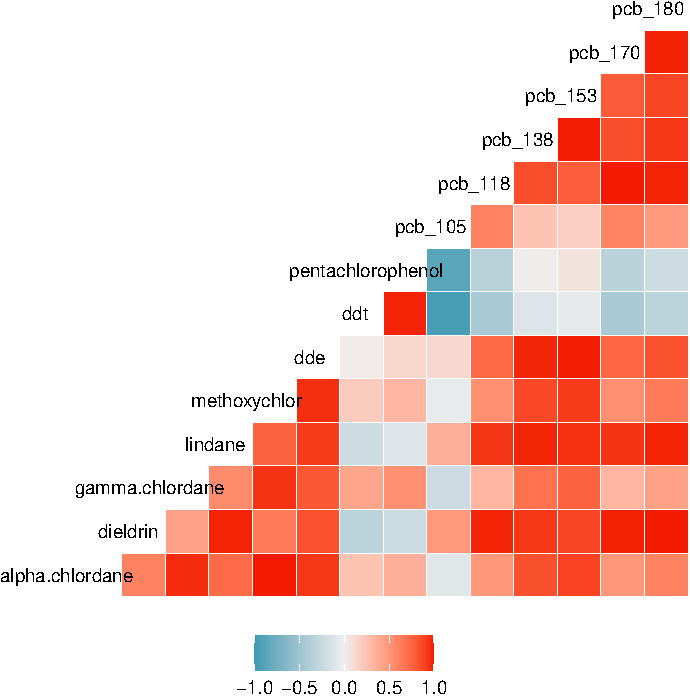
\includegraphics{hargarten_wheeler_files/figure-latex/dataCorr-1.pdf} 

}

\caption{\label{fig::dataCorr} Heat map of the correlations using the fourteen observed chemical logarithmic concentrations in dataset simdata87 can be analyzed with the package miWQS. The heat map was generated using the GGally package.}\label{fig:dataCorr}
\end{figure}


Chemical exposure patterns often differ between individuals due to
demographics and other confounders. The additional covariates
\(\boldsymbol{Z}\) can be represented as a vector, data frame, or
matrix. For example, the element \code{Z.sim} in the list
\code{simdata87} is a matrix that contains an individual's age, sex
(Female/Male), ethnicity (Hispanic/Non-Hispanic), and race
(White/non-White). Some statistics of the covariates are shown below.

\begin{Schunk}
\begin{Sinput}
> summary(simdata87$Z.sim[, "Age"])
\end{Sinput}
\begin{Soutput}
   Min. 1st Qu.  Median    Mean 3rd Qu.    Max. 
 0.0224  2.4909  3.7443  3.7176  4.8805  7.9771 
\end{Soutput}
\begin{Sinput}
> apply(simdata87$Z.sim[, -1], 2, table)
\end{Sinput}
\begin{Soutput}
  Female Hispanic Non-Hispanic_Others
0    611      670                 766
1    389      330                 234
\end{Soutput}
\end{Schunk}

The univariate outcome shared among the components, \(y\), may be
continuous, count-based, or binary; it is represented as a numeric
vector or a factor in R. The mean of the outcome, \(\xi\), relates the
covariates and chemicals by a link function \emph{g()} as in generalized
linear models. Continuous, count-based, and binary outcomes all commonly
arise in public health and medicine. First, exposure to a mixture of
chemicals may be associated with continuous health outcomes, such as
body mass index (BMI), systolic blood pressure, or cholesterol. When
\(y\) is continuous, we assume a Gaussian distribution using an identity
link. Next, count health outcomes may arise in evaluations of
socioeconomic data or environmental exposures in census regions. When
\(y\) is a count, we assume a Poisson distribution with a log link and
use an offset if a rate is modeled. Finally, binary health outcomes are
common in environmental exposure data and in case-control studies. When
\(y\) is binary, we assume a Bernoulli distribution using a logistic
link. In our dataset, the \code{y.scenario} element of \code{simdata87}
is binary. Suppose that \code{y.scenario} consists of cancer cases
(represented by 1) and controls (represented by 0). The table below
shows that 457 individuals (45.7\%) are diagnosed with cancer.

\begin{Schunk}
\begin{Sinput}
> cat("Counts")
> table(simdata87$y.scenario)
\end{Sinput}
\begin{Soutput}
Counts
  0   1 
543 457 
\end{Soutput}
\end{Schunk}

In our dataset--\code{simdata87}--we will like to answer the following
research questions: (1) Is the mixture of correlated chemicals
associated with cancer; (2) if so, what are the important chemicals? In
the examples that follow, we will use both non-missing and missing
chemical concentrations that are handled in four different ways.

\hypertarget{example-1-wqs-regression-using-complete-data}{%
\section{Example 1: WQS regression using complete
data}\label{example-1-wqs-regression-using-complete-data}}

WQS regression allows us to estimate the effect of a chemical mixture on
the disease while parsimoniously selecting important components
\citep{carricoCharacterizationWeightedQuantile2014, czarnotaAssessmentWeightedQuantile2015, genningsCohortStudyEvaluation2013, hargartenAccountingUncertaintyDue2020}.
Briefly, WQS regression was designed to select components in
environmental exposure analysis. The correlated components are scored
into quantiles. Let \(q_{ij}\) represent the values of the \(jth\)
chemical exposed in the \(ith\) subject. Ideally, the data should be
randomly split into a training dataset and validation dataset. While the
training set is used to create the WQS index, the validation dataset is
used to assess the association of the weighted index with the outcome.
Yet, small datasets should not be split as splitting them may result in
inadequate power to detect a signal.

In the training dataset, the weights are estimated from \(B\)
bootstrapped samples of size \(n_T\) to form the weighted index. Each
bootstrap sample is used to estimate the unknown weights \(w_j\) that
maximize the likelihood in the following nonlinear model:
\[g( \xi_{i} ) = \beta_{0b}^{(T)} + \beta_{1b}^{(T)} \cdot \left( \sum_{j=1}^c w_{jb}\cdot q_{ij} \right) + \boldsymbol{z}_{ib}^{\prime} \cdot \boldsymbol{\theta}^{(T)}, \]
subject to
\[\beta_{1b}^{(T)} >0, \; 0 \le w_{jb} \le 1, \; \text{and} \; \sum_{j=1}^c w_{jb} = 1 \]
for the \(b^{\text{th}}\) bootstrap sample. The parameters are as
follows: \(\beta_{0b}^{(T)}\) is the intercept, \(\beta_{1b}^{(T)}\) is
the overall mixture effect, and \(\boldsymbol{\theta}\) are the
covariate parameters. The term
\(\left( \sum_{j=1}^c w_{jb}\cdot q_{ij} \right)\) represents the
weighted index of the \(c\) chemicals of interest. The parameters in the
training dataset are represented with superscript \(T\). The final
weight estimate \(\bar{w_j}\) is calculated as an average of the
bootstrap estimates \(\hat{w}_{jb}\) for the jth chemical:
\[\bar{w_j} = \frac{1}{B} \sum_{b=1}^B \hat{w}_{jb}.\]

A constraint is placed on \(\beta_{1b}^{(T)}\) to allow for
interpretation of the index
\citep{carricoCharacterizationWeightedQuantile2014}. Often, exploratory
single-chemical analyses, shown in
\protect\hyperlink{Appendix-1}{Appendix 1}, show that some components in
the mixture have a negative association with the outcome, while others
have a positive association. In environmental risk analysis, researchers
are often interested in a positive association between the mixture of
components and an adverse health outcome. However, if a researcher
hypothesizes that the overall mixture is protective of the outcome, the
constraint \(\beta_{1b}^{(T)} > 0\) should be switched to
\(\beta_{1b}^{(T)} < 0\).

Then, the weighted quantile index score of the \(i^{\text{th}}\)
individual is specified as:
\({WQS}_{i} = \sum_{j=1}^{c} \bar w_j \cdot q_{ij}\), which uses the
quantiles in the validation dataset. In the validation dataset, the
significance of the WQS parameter (\(\beta_{1}^{(V)}\)) can be
determined from:
\[ g(\xi_{i}) = \beta_{0}^{(V)} + \beta_{1}^{(V)} WQS_i + \boldsymbol{z}_i' \cdot \boldsymbol{\theta}^{(V)}, \]
where superscript \(V\) represents the regression coefficients in the
validation dataset. While \(\beta_{1}^{(V)}\) describes the effect of
the chemical mixture on the health outcome, the mean weight \(\bar w_j\)
identifies the relative importance that chemical \(j\) imposes on the
outcome
\citep{carricoCharacterizationWeightedQuantile2014, czarnotaAssessmentWeightedQuantile2015, genningsCohortStudyEvaluation2013, hargartenAccountingUncertaintyDue2020}.

The \code{estimate.wqs()} function performs WQS regression in the
\pkg{miWQS} package. The data as specified in
\protect\hyperlink{Data-structure}{Data structure} section are placed in
the first three arguments. The \code{y} argument takes the outcome, like
\code{simdata87\$y.scenario}. As \code{y.scenario} is binary, the
binomial distribution is specified by setting the \code{family} argument
to \code{"binomial"}. The \code{X} argument takes the chemicals of
interest, like \code{simdata87\$X.true}. If \code{X} contains
\code{NA}'s (that represents missing values), the BDL values are placed
in the first quantile by default (see
\protect\hyperlink{Example-2}{Example 2}). Any additional demographic
covariates, like \code{simdata87\$Z.sim}, are placed into the \code{Z}
argument. If no covariates are present, set \code{Z} to \code{NULL}. The
\code{b1.pos} argument controls whether the overall mixture effect,
\(\beta_1^{(T)}\), is positively related to the outcome. A way to decide
the direction is to use the \code{analyze.individually()} function,
which is described in more detail in
\protect\hyperlink{Appendix-1}{Appendix 1}. In our dataset, we assume a
positive relationship between the mixture and an outcome; we
consequently set \code{b1.pos} to \code{TRUE}. The
\code{proportion.train} argument specifies the proportion of data given
to the training dataset. As the sample size of our example dataset is
large (n = 1000), we will use 50\% of the data to train. The \code{B}
argument is the number of bootstraps used to estimate the weights
\(w_j\)'s.

We set a seed to ensure reproducibility as we bootstrapped the data. The
execution of the \code{estimate.wqs()} function creates an object of
class \code{wqs}, and printing it answers the main research questions.

\begin{Schunk}
\begin{Sinput}
> set.seed(50679)
> wqs.eg1 <- estimate.wqs(
+   y = simdata87$y.scenario, X = simdata87$X.true, Z = simdata87$Z.sim,
+   proportion.train = 0.5,
+   n.quantiles = 4,
+   place.bdls.in.Q1 = FALSE,
+   B = 100, 
+   b1.pos = TRUE, 
+   signal.fn = "signal.converge.only",
+   family = "binomial",
+   verbose = FALSE
+ )
\end{Sinput}
\begin{Soutput}
#> No missing values in matrix detected. Regular quantiles computed.
\end{Soutput}
\begin{Sinput}
> wqs.eg1
\end{Sinput}
\begin{Soutput}

Odd Ratios & 95% CI (N.valid = 500) 
                     Odds Ratio  SE.OR                95% CI  P-value
(Intercept)               0.142   1.51  0.142 (0.063, 0.320)   <0.001
Age                       0.950   1.06  0.950 (0.854, 1.056)    0.339
Female                    0.947   1.22  0.947 (0.646, 1.388)    0.780
Hispanic                  1.580   1.23  1.578 (1.059, 2.352)    0.025
Non.Hispanic_Others       1.030   1.25  1.034 (0.671, 1.593)    0.880
WQS                       3.660   1.25  3.663 (2.372, 5.659)   <0.001
AIC:  660.7468 

All (100) bootstraps have converged. 

 Weights Adjusted by signal.converge.only using N.train = 500 observations: 
              ddt            pcb_105            pcb_170            pcb_138  
           0.3905             0.2413             0.1105             0.1014  
          pcb_153                dde            pcb_118  pentachlorophenol  
           0.0344             0.0339             0.0217             0.0216  
          lindane    gamma.chlordane       methoxychlor    alpha.chlordane  
           0.0200             0.0138             0.0043             0.0028  
          pcb_180           dieldrin  
           0.0024             0.0014  
Important chemicals defined as mean weights > 1/14~0.071. 
\end{Soutput}
\end{Schunk}

An increase in the chemical mixture is associated with an increase in
the odds of being diagnosed with cancer by 3.66. The
\code{coef(wqs.eg1)} gives us estimates on the logit scale of
coefficients in the validation model. We identify chemicals in the
mixture as important if their weight estimates are greater than the
reciprocal of the number of chemicals. Alpha-chlordane, PCB 153, PCB
105, and p,p-DDE approximately constitute 88\% of the effect in the
index. Thus, these three chemicals are associated with increased cancer
risk. The weight estimates are directly extracted with
\code{wqs.eg1\$processed.weights}. The Akaike information criterion
(AIC) is used as the goodness-of-fit measure of the WQS model and is
directly computed using \code{AIC(wqs.eg1\$fit)}.

Plotting a WQS object gives a list of histograms: the distributions of
the weight estimates, the overall effect of the mixture, and the WQS
index score \citep{wickhamGgplot2ElegantGraphics2016}.

\begin{Schunk}
\begin{Sinput}
> eg1.plots <- plot(wqs.eg1)
> names(eg1.plots)
\end{Sinput}
\begin{Soutput}
[1] "hist.weights" "hist.beta1"   "hist.WQS"    
\end{Soutput}
\end{Schunk}

Commonly, researchers look at distributions of the weight estimates to
determine which chemicals are important in the mixture (Figure
\ref{fig::histWeight}). Looking at the histograms for complete WQS data,
most chemicals have no effect among all bootstraps. However, this panel
of histograms indicates that alpha-chlordane, p,p-DDE, PCB 153, and PCB
105 are important, which agrees with our above statistical analysis.


\begin{figure}[h]

{\centering 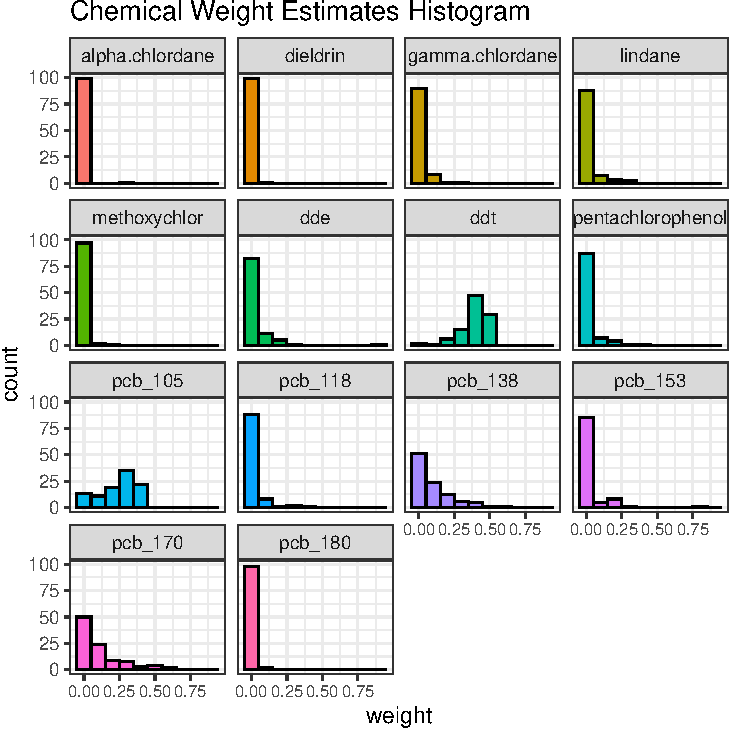
\includegraphics{hargarten_wheeler_files/figure-latex/histWeight-1.pdf} 

}

\caption{\label{fig::histWeight} Histograms of chemical weight estimates across 100 bootstraps for Example 1 to select important chemicals. Weight estimates are constrained to be between zero and one.}\label{fig:histWeight}
\end{figure}


The second histogram provides us insight into the distribution of the
overall effect of the mixture on the outcome, \(\beta^{(T)}_1\), across
the bootstraps (Figure \ref{fig::histB1}). Most bootstraps indicate that
the chemical mixture is not associated with the outcome (median around
1).


\begin{figure}[h]

{\centering 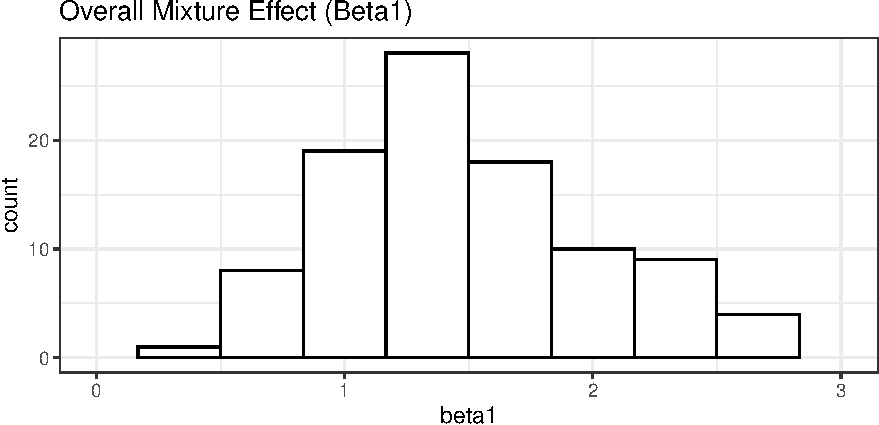
\includegraphics{hargarten_wheeler_files/figure-latex/histB1-1.pdf} 

}

\caption{\label{fig::histB1} Histogram of overall chemical effect in the training dataset across 100 bootstraps for Example 1. Its constraint is governed by the b1.pos argument in the estimate.wqs() function. In the simdata87 dataset, the overall mixture is constrained to have a positive association with cancer. Most bootstraps indicate that the chemical mixture is not associated with the outcome.}\label{fig:histB1}
\end{figure}


The third histogram shows us the distribution of the weighted quantile
sum. Given constraints placed on the weights, WQS is a continuous index
between zero and the number of quantiles minus 1 (given by the
\code{n.quantiles} argument in \code{estimate.wqs()} ) (Figure
\ref{fig::histWQS}). In our example, the number of quantiles is four.
Across the bootstrap samples, most values of the chemical mixture are
between one and two.


\begin{figure}[h]

{\centering 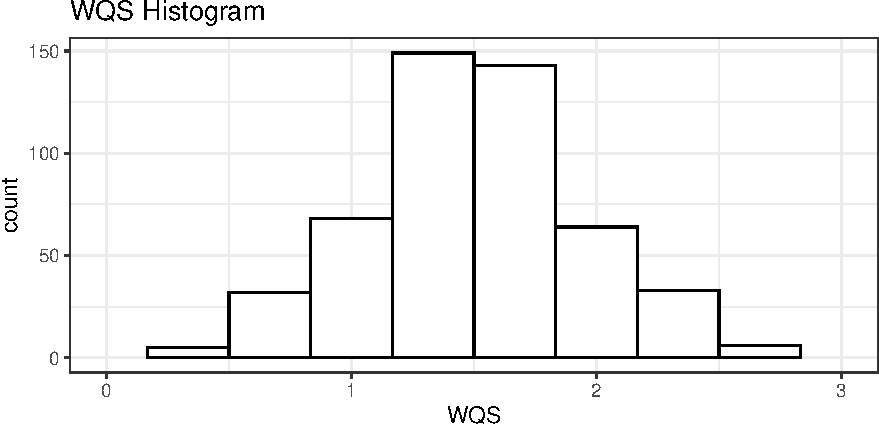
\includegraphics[width=0.85\linewidth]{hargarten_wheeler_files/figure-latex/histWQS-1.pdf} 

}

\caption{\label{fig::histWQS} Histogram of the weighted quantile sum (WQS) using validation quantiles for Example 1 to show where most values of the chemical mixture lie.}\label{fig:histWQS}
\end{figure}


\hypertarget{example-2-bdlq1-approach-on-interval-censored-data}{%
\section{Example 2: BDLQ1 approach on interval-censored
data}\label{example-2-bdlq1-approach-on-interval-censored-data}}

\hypertarget{bdlq1-approach}{%
\subsection{BDLQ1 approach}\label{bdlq1-approach}}

Unlike \protect\hyperlink{Example-1}{Example 1}, many studies contain
partially observed chemical concentrations that are measured to
different detection limits. One approach to use WQS with missing data is
to place the BDL values into the first quantile (BDLQ1), and to score
the observed component values in the remaining quantiles. The
\code{make.quantile.matrix()} function demonstrates this approach by
creating \code{n.quantiles} quantiles from a matrix argument \code{X}.
If \code{X} is completely observed, regular quantiles are made; however,
if the first values in \code{X} are missing, they are placed in the
first quantile. For example, suppose we are interested in making four
quantiles of 14 chemicals using 1,000 subjects in our dataset. If we use
the completely observed concentrations found in \code{X.true} element of
\code{simdata87}, regular quantiles for all 14 chemicals are made with
the following number of individuals per quantile.

\begin{Schunk}
\begin{Sinput}
> q <- make.quantile.matrix(
+   X = simdata87$X.true,
+   n.quantiles = 4
+   )
\end{Sinput}
\begin{Soutput}
#> No missing values in matrix detected. Regular quantiles computed.
\end{Soutput}
\begin{Sinput}
> apply(q, 2, table)
\end{Sinput}
\begin{Soutput}
  [,1] [,2] [,3] [,4] [,5] [,6] [,7] [,8] [,9] [,10] [,11] [,12] [,13] [,14]
0  250  250  250  250  250  250  250  250  250   250   250   250   250   250
1  250  250  250  250  250  250  250  250  250   250   250   250   250   250
2  250  250  250  250  250  250  250  250  250   250   250   250   250   250
3  250  250  250  250  250  250  250  250  250   250   250   250   250   250
\end{Soutput}
\end{Schunk}

However, if the chemical concentrations are incomplete (with the missing
values indicated as \code{NA}'s), the BDLQ1 approach works as follows.
Suppose we wish to make quartiles of the \code{X.bdl} matrix in our
dataset, where each chemical has 100 BDL concentrations. Using BDLQ1,
the 100 observations are placed into the first quartile, and the
remaining quartiles are evenly split in which each contains 900/3 = 300
observations. The number of individuals in each quartile of each
chemical, and the total number of missing values in each chemical are
shown below. Note that the first row of the matrix matches the total
number of missing values (100).

\begin{Schunk}
\begin{Sinput}
> q <- make.quantile.matrix(
+   simdata87$X.bdl, 
+   n.quantiles = 4, 
+   verbose = TRUE
+   )
\end{Sinput}
\begin{Soutput}
#> All BDLs are placed in the first quantile
\end{Soutput}
\begin{Soutput}
##> Summary of Quantiles 
  [,1] [,2] [,3] [,4] [,5] [,6] [,7] [,8] [,9] [,10] [,11] [,12] [,13] [,14]
0  100  100  100  100  100  100  100  100  100   100   100   100   100   100
1  300  300  300  300  300  300  300  300  300   300   300   300   300   300
2  300  300  300  300  300  300  300  300  300   300   300   300   300   300
3  300  300  300  300  300  300  300  300  300   300   300   300   300   300
##> Total Number of NAs--Q1 (The first row) should match.
100 100 100 100 100 100 100 100 100 100 100 100 100 100
\end{Soutput}
\end{Schunk}

The number of individuals in the first quantile in BDLQ1 increases if
more BDL values exist. For instance, \code{X.80} substitutes 800 values
for each chemical from \code{simdata87\$X.true} to be missing BDL.
Applying the BDLQ1 approach to \code{X.80}, all 800 values are placed
into the first quartile, while roughly \(200/3 \approx 66\) values are
placed in remaining quartiles.

\begin{Schunk}
\begin{Sinput}
> q <- make.quantile.matrix(X.80, n.quantiles = 4, verbose = TRUE)
\end{Sinput}
\begin{Soutput}
#> All BDLs are placed in the first quantile
\end{Soutput}
\begin{Soutput}
##> Summary of Quantiles 
  [,1] [,2] [,3] [,4] [,5] [,6] [,7] [,8] [,9] [,10] [,11] [,12] [,13] [,14]
0  800  800  800  800  800  800  800  800  800   800   800   800   800   800
1   67   67   67   67   67   67   67   67   67    67    67    67    67    67
2   66   66   66   66   66   66   66   66   66    66    66    66    66    66
3   67   67   67   67   67   67   67   67   67    67    67    67    67    67
##> Total Number of NAs--Q1 (The first row) should match.
800 800 800 800 800 800 800 800 800 800 800 800 800 800
\end{Soutput}
\end{Schunk}

Instead of quantiles, we could also categorize the chemicals into
deciles by changing the \code{n.quantiles} argument to ten. Suppose now
that we wish to form deciles in \code{simdata87\$X.bdl}. The first 100
BDL values are placed in the first decile, while the remaining 900 are
evenly spread out in the remaining nine deciles (900/9 = 100).

\begin{Schunk}
\begin{Sinput}
> q <- make.quantile.matrix(simdata87$X.bdl, n.quantiles = 10, verbose = TRUE)
\end{Sinput}
\begin{Soutput}
#> All BDLs are placed in the first quantile
\end{Soutput}
\begin{Soutput}
##> Summary of Quantiles 
  [,1] [,2] [,3] [,4] [,5] [,6] [,7] [,8] [,9] [,10] [,11] [,12] [,13] [,14]
0  100  100  100  100  100  100  100  100  100   100   100   100   100   100
1  100  100  100  100  100  100  100  100  100   100   100   100   100   100
2  100  100  100  100  100  100  100  100  100   100   100   100   100   100
3  100  100  100  100  100  100  100  100  100   100   100   100   100   100
4  100  100  100  100  100  100  100  100  100   100   100   100   100   100
5  100  100  100  100  100  100  100  100  100   100   100   100   100   100
6  100  100  100  100  100  100  100  100  100   100   100   100   100   100
7  100  100  100  100  100  100  100  100  100   100   100   100   100   100
8  100  100  100  100  100  100  100  100  100   100   100   100   100   100
9  100  100  100  100  100  100  100  100  100   100   100   100   100   100
##> Total Number of NAs--Q1 (The first row) should match.
100 100 100 100 100 100 100 100 100 100 100 100 100 100
\end{Soutput}
\end{Schunk}

The BDLQ1 method has been used in single-chemical analyses
\citep{metayerExposureHerbicidesHouse2013, wardResidentialLevelsPolybrominated2014, wardResidentialExposurePolychlorinated2009}
and WQS \citep{hargartenAccountingUncertaintyDue2020}. However, it has
not been coded in other WQS packages to the best of our knowledge.

\hypertarget{wqs-analysis}{%
\subsection{WQS analysis}\label{wqs-analysis}}

The BDLQ1 method works because WQS regression uses quantile scores from
each chemical in the mixture. At this step, the \code{estimate.wqs()}
function calls the \code{make.quantile.matrix()} function. Setting the
argument \code{place.bdls.in.Q1} to \code{TRUE} allows us to use the WQS
regression in conjunction with the BDLQ1 method. Yet, if the \code{X}
argument contains any missing values, the BDLQ1 approach is
automatically used. The incomplete data \code{X.bdl} is now assigned to
the chemical mixture \code{X} argument. The remaining arguments in
\code{estimate.wqs()} are the same as in
\protect\hyperlink{Example-1}{Example 1}. Printing the resulting object
answers the research questions of interest. The research aims are to
determine the association of the mixture with cancer and to find the
important chemicals (if the association exists).

\begin{Schunk}
\begin{Sinput}
> set.seed(50679)
> wqs.BDL <- estimate.wqs(
+   y = simdata87$y.scenario, X = simdata87$X.bdl, Z = simdata87$Z.sim,
+   proportion.train = 0.5, 
+   n.quantiles = 4,
+   place.bdls.in.Q1 = TRUE,
+   B = 100,
+   b1.pos = TRUE, 
+   signal.fn = "signal.converge.only",
+   family = "binomial",
+   verbose = FALSE
+ )
\end{Sinput}
\begin{Soutput}
#> All BDLs are placed in the first quantile
\end{Soutput}
\begin{Sinput}
> wqs.BDL
\end{Sinput}
\begin{Soutput}

Odd Ratios & 95% CI (N.valid = 500) 
                     Odds Ratio  SE.OR                95% CI  P-value
(Intercept)               0.214   1.52  0.214 (0.094, 0.483)   <0.001
Age                       0.952   1.05  0.952 (0.858, 1.057)    0.356
Female                    0.926   1.21  0.926 (0.636, 1.349)    0.688
Hispanic                  1.560   1.22  1.558 (1.052, 2.306)    0.027
Non.Hispanic_Others       1.050   1.24  1.052 (0.687, 1.612)    0.816
WQS                       2.360   1.21  2.358 (1.626, 3.420)   <0.001
AIC:  677.0172 

1 bootstrap(s) have failed to converged. Those are: 
[1] 60

 Weights Adjusted by signal.converge.only using N.train = 500 observations: 
          pcb_105  pentachlorophenol    gamma.chlordane    alpha.chlordane  
           0.2575             0.2548             0.1622             0.0699  
          pcb_153            pcb_138                ddt            lindane  
           0.0658             0.0606             0.0378             0.0349  
     methoxychlor            pcb_118                dde            pcb_170  
           0.0180             0.0128             0.0075             0.0066  
         dieldrin            pcb_180  
           0.0065             0.0051  
Important chemicals defined as mean weights > 1/14~0.071. 
\end{Soutput}
\end{Schunk}

An increase in one-quartile of the chemical mixture is associated with
an increase in the odds of obtaining cancer by 2.36. Compared to the
complete case analysis, PCB 105 and alpha-chlordane are still important,
but DDT, PCB 170, and methoxychlor are also important in the BDLQ1
analysis. As we forced some complete concentrations
\code{simdata87\$X.true} to be BDL values in creating
\code{simdata87\$X.bdl}, we used AIC to compare fit between the two WQS
models in Examples \protect\hyperlink{Example-1}{1} and
\protect\hyperlink{Example-2}{2}. Intuitively, a WQS model using the
BDLQ1 approach (AIC: 677) fits the data worse than a WQS model using
complete data (AIC: 661).

\hypertarget{example-3-bootstrapping-interval-censored-data}{%
\section{Example 3: Bootstrapping interval-censored
data}\label{example-3-bootstrapping-interval-censored-data}}

An alternative to the BDLQ1 approach is to perform multiple imputation
of the missing chemical values by bootstrapping
\citep{lubinEpidemiologicEvaluationMeasurement2004}. Given completely
observed covariates \(z_{i1},\ldots z_{\text{ik}}\) in \(i=1, ...n\)
subjects exposed to \(j=1,...c\) chemicals, an independent log-normal
distribution for each chemical \(j\) with mean \(\mu_{j}\) and variance
\(\sigma^2_j\) is assumed:
\[\log(x_{ij})| z_1 \cdots z_p \sim ^{indep} N \left(\mu_j = \boldsymbol{z}_i^\prime \cdot \boldsymbol{\gamma}_j, \sigma^2_j \right) .\]
Let \(f(.)\) denote the normal probability density function and \(F(.)\)
denote its cumulative distribution function. For each chemical \(j\),
the dataset is bootstrapped \(K\) times to form \(K\) complete datasets.
As each bootstrap \(b\) is sampled with replacement from the original
data, the number of times the \(i^{\text{th}}\) subject is selected for
\(j^{\text{th}}\) chemical is represented by \(w_{\text{ij}}\). The log
likelihood function for the bootstrap data in \(j^{\text{th}}\) chemical
is given by:

\[l(\boldsymbol{\gamma}_{j}, \sigma^2_j) = \sum_{i=1}^{n_{0j}} w_{ij} * \log \left [ P \left (0 < X_{ij} < DL_{j}; \boldsymbol{z}_i^\prime \cdot \boldsymbol{\gamma}_{j},\sigma^2_j \right) \right ] + \sum_{i=n_{0j}+1}^n \log \left[ f( x_{ij}; \boldsymbol{z}_i^\prime \cdot \boldsymbol{\gamma}_{j}, \sigma^2_j) \right],\]
where \(n_{0j}\) represents the number of BDL values for chemical \(j\).
The estimates that maximize the log likelihood are
\(\left({\tilde{\boldsymbol{\gamma}}}_{j},\tilde{\sigma}^2_j \right)\).
Then, the BDL values are imputed by the following method. We generate an
independent and identically distributed uniform sample between zero and
\(F \left( \log(DL_j); \boldsymbol{z}_i^\prime \cdot \tilde{\boldsymbol{\gamma}}_j, \tilde{\sigma}^2_j \right )\).
Then, we assign value \(F^{- 1} \left( u_{\text{ij}} \right)\) for each
missing value \(x_{\text{ij}}\) below the detection limit of the
\(j^{\text{th}}\) chemical \(DL_{j}\)
\citep{lubinEpidemiologicEvaluationMeasurement2004}. These imputed
values are joined with the observed ones to form one complete set of
exposures for the \(j^{\text{th}}\) chemical. The \code{impute.Lubin()}
function performs multiple imputation by bootstrapping for one chemical.
For instance, suppose we wish to impute the dieldrin concentrations BDL
twice (\(K = 2\)) in \code{simdata87} by bootstrapping using the
following covariates: childhood age, sex, and child race/ethnicity. The
dieldrin concentrations are found in the first column of \code{X.bdl} in
\code{simdata87} dataset (e.g.~\code{simdata87\$X.bdl[ , 1]}), and the
detection limit of dieldrin is in the first entry in \code{DL} element
(e.g.~\code{simdata87\$DL[1]}). The \code{chemcol} argument is a numeric
vector of chemical concentrations that we wish to impute
(e.g.~\code{simdata87\$X.bdl[ , 1]}). The \code{dlcol} argument is the
detection limit of the chemical (e.g.~\code{simdata87\$DL[1]}). The
\code{Z} argument contains any covariates used in the imputation
(e.g.~\code{simdata87\$Z.sim} and \code{simdata87\$y.scenario}). We
included the outcome in the imputation of BDL values because its
omission assumes that it is not associated with the BDL values and
thereby bias the subsequent WQS coefficients towards zero
\citep{forerMissingData2014, barnardMultipleImputation2015}. The
\code{K} argument is the number of imputed datasets (e.g.~\code{2}).

\begin{Schunk}
\begin{Sinput}
> set.seed(472195)
> answer <- impute.Lubin(
+   chemcol = simdata87$X.bdl[, 1],
+   dlcol = simdata87$DL[1],
+   Z = cbind(simdata87$y.scenario, simdata87$Z.sim), 
+   K = 2
+ )
> summary(answer$imputed_values)
\end{Sinput}
\begin{Soutput}
     Imp.1              Imp.2         
 Min.   :       0   Min.   :       0  
 1st Qu.:      11   1st Qu.:      11  
 Median :     125   Median :     125  
 Mean   :   44099   Mean   :   44099  
 3rd Qu.:    1682   3rd Qu.:    1682  
 Max.   :17354723   Max.   :17354723  
\end{Soutput}
\end{Schunk}

The \code{answer\$imputed\_values} is a matrix with rows of 1000
subjects and two columns consisting of the imputed dieldrin
concentrations. Since most concentrations are observed, the summaries of
the two datasets should look the same. However, if we look at BDL
values, the two imputed datasets are different, and both are under the
detection limit (0.924).

\begin{Schunk}
\begin{Sinput}
> cat("Summary of BDL Values \n")
> imp <- answer$imputed_values[, 1] < simdata87$DL[1]
> summary(answer$imputed_values[imp, ])
\end{Sinput}
\begin{Soutput}
Summary of BDL Values 
     Imp.1             Imp.2         
 Min.   :0.00124   Min.   :0.001417  
 1st Qu.:0.04579   1st Qu.:0.057819  
 Median :0.22420   Median :0.201560  
 Mean   :0.32314   Mean   :0.272618  
 3rd Qu.:0.59102   3rd Qu.:0.444859  
 Max.   :0.91690   Max.   :0.854974  
\end{Soutput}
\end{Schunk}

More than one chemical often needs to be imputed in many studies. To
implement the bootstrap approach, we use the \code{impute.boot()}
function, which repeatedly executes the \code{impute.Lubin()} function.
In \code{simdata87}, now suppose that we wish to impute the \code{X.bdl}
matrix twice by bootstrapping using the covariates (\code{Z}) of age,
sex, and race/ethnicity. The \code{X} argument takes a matrix with
incomplete data, like \code{simdata87\$X.bdl}. The next argument,
\code{DL}, takes the detection limits of \code{X} as a numeric vector,
like \code{simdata87\$DL}. The \code{K} and \code{Z} arguments are
exactly the same as in \code{impute.Lubin()}. A seed is set before the
function to ensure that the same bootstrap samples are selected for each
chemical. The function returns a list \code{l.boot}.

\begin{Schunk}
\begin{Sinput}
> set.seed(472195)
> l.boot <- impute.boot(
+   X = simdata87$X.bdl, 
+   DL = simdata87$DL, 
+   Z = cbind(simdata87$y.scenario, simdata87$Z.sim), 
+   K = 2
+   )
\end{Sinput}
\begin{Soutput}
#> Check: The total number of imputed values that are above the detection limit is 0.
\end{Soutput}
\begin{Sinput}
> results.Lubin <- l.boot$X.imputed
\end{Sinput}
\end{Schunk}

The \code{X.imputed} element of \code{l.boot} saves the imputed chemical
values as an array, where the first dimension is the number of subjects
(\(n\)), the second is the number of chemicals (\(c\)), and the third is
the number of imputed datasets (\(K\)). The sample minima, fifth
percentile (\code{P.5}), means, and maxima of the chemicals are
calculated in each imputed dataset (by the function \code{f()}). As the
two imputed datasets are different, the application of MI should yield
different parameter estimates.

\begin{Schunk}
\begin{Sinput}
> apply(results.Lubin, 2:3, f)
\end{Sinput}
\begin{Soutput}
, , Imp.1

     alpha-chlordane     dieldrin gamma-chlordane   lindane methoxychlor
min     1.239744e-03 5.214163e-02        14.85745  3.122209     16.13658
P.5     2.257984e-01 2.016689e+00        25.79766  7.147067     35.19478
mean    4.409885e+04 4.331448e+02        49.38257 17.214769     83.45674
max     1.735472e+07 4.867330e+04       139.33689 75.360498    316.07141
              dde        ddt pentachlorophenol     pcb_105     pcb_118
min  4.500939e-02   1.532625          1.604183   0.1372503   0.4547588
P.5  8.736265e-01   3.544432          3.923535   1.1031301   1.4373202
mean 2.546607e+03  16.122825         20.262419  16.4815577   9.7025958
max  3.835674e+05 178.853960        285.229348 400.3601114 142.2619560
          pcb_138      pcb_153     pcb_170     pcb_180
min    0.08042499   0.03363274   0.7155792   0.1741525
P.5    0.80147195   0.47230663   2.5599230   0.7335900
mean  12.63094227  13.82089093  11.6125246   8.4248157
max  269.09903138 383.79850341 115.2060922 203.8593938

, , Imp.2

     alpha-chlordane     dieldrin gamma-chlordane   lindane methoxychlor
min     1.417111e-03     0.117659        14.57128  3.690147     15.35223
P.5     2.024978e-01     2.276511        25.50909  6.751412     36.11395
mean    4.409884e+04   433.153356        49.36521 17.201076     83.39251
max     1.735472e+07 48673.296171       139.33689 75.360498    316.07141
              dde         ddt pentachlorophenol     pcb_105     pcb_118
min  3.502864e-02   0.9292443          1.299465   0.1512212   0.4144885
P.5  9.079915e-01   3.3656892          3.959147   1.0578307   1.3154884
mean 2.546614e+03  16.1134725         20.250618  16.4788855   9.6934267
max  3.835674e+05 178.8539599        285.229348 400.3601114 142.2619560
         pcb_138      pcb_153     pcb_170      pcb_180
min    0.2291489   0.08258941   0.4825019   0.05475401
P.5    0.8403295   0.52882557   2.5113298   0.69996133
mean  12.6359530  13.82390718  11.6064361   8.42308671
max  269.0990314 383.79850341 115.2060922 203.85939377
\end{Soutput}
\end{Schunk}

Next, we implement WQS regression on the two complete datasets, which
are saved in the \code{results.Lubin} object. Instead of performing WQS
on one dataset as in Examples \protect\hyperlink{Example-1}{1} and
\protect\hyperlink{Example-2}{2}, the \code{do.many.wqs()} function
repeatedly executes WQS regression on each dataset. The arguments for
the \code{do.many.wqs()} function are the same as the
\code{estimate.wqs()} function, with one exception. The \code{X.imputed}
argument now is an array of the imputed chemical values, which has three
dimensions: \emph{n} subjects, \emph{c} chemicals, and \emph{K} imputed
datasets. This array is the output from the \code{impute.boot()}
function: \code{results.Lubin}.

\begin{Schunk}
\begin{Sinput}
> set.seed(50679)
> boot.wqs <- do.many.wqs(
+   y = simdata87$y.scenario, X.imputed = results.Lubin, Z = simdata87$Z.sim,
+   proportion.train = 0.5, 
+   n.quantiles = 4, 
+   B = 100,
+   b1.pos = TRUE,
+   signal.fn = "signal.converge.only",
+   family = "binomial"
+ )
\end{Sinput}
\begin{Soutput}
#> Sample size: 1000; Number of chemicals: 14; 
Number of completed datasets: 2; Number of covariates modeled:  4
\end{Soutput}
\end{Schunk}

The \code{do.many.wqs()} function returns list and matrix versions of
the output generated from the \code{estimate.wqs()} function. The
\code{wqs.imputed.estimates} element of the \code{boot.wqs} list is a
three-dimensional array that gives the WQS estimates for each imputed
dataset. The first dimension consists of the total number parameters in
the WQS model. The second dimension consists of two columns: the mean
and standard deviation of estimates. The third dimension is the \emph{K}
imputation draws.

\begin{Schunk}
\begin{Sinput}
> formatC(boot.wqs$wqs.imputed.estimates, format = "fg", flag = "#", digits = 3)
\end{Sinput}
\begin{Soutput}
, , Imputed.1

                    Estimate  Std.Error
alpha.chlordane     "0.00285" "0.0285" 
dieldrin            "0.00139" "0.0101" 
gamma.chlordane     "0.0138"  "0.0442" 
lindane             "0.0200"  "0.0525" 
methoxychlor        "0.00429" "0.0244" 
dde                 "0.0339"  "0.104"  
ddt                 "0.391"   "0.0936" 
pentachlorophenol   "0.0216"  "0.0628" 
pcb_105             "0.241"   "0.129"  
pcb_118             "0.0217"  "0.0697" 
pcb_138             "0.101"   "0.131"  
pcb_153             "0.0344"  "0.0986" 
pcb_170             "0.110"   "0.149"  
pcb_180             "0.00236" "0.0114" 
(Intercept)         "-1.95"   "0.415"  
Age                 "-0.0516" "0.0540" 
Female              "-0.0546" "0.195"  
Hispanic            "0.456"   "0.204"  
Non.Hispanic_Others "0.0333"  "0.221"  
WQS                 "1.30"    "0.222"  

, , Imputed.2

                    Estimate  Std.Error
alpha.chlordane     "0.00424" "0.0185" 
dieldrin            "0.0392"  "0.0801" 
gamma.chlordane     "0.00843" "0.0257" 
lindane             "0.00191" "0.0119" 
methoxychlor        "0.0103"  "0.0518" 
dde                 "0.0767"  "0.114"  
ddt                 "0.148"   "0.159"  
pentachlorophenol   "0.272"   "0.163"  
pcb_105             "0.156"   "0.114"  
pcb_118             "0.0102"  "0.0302" 
pcb_138             "0.213"   "0.193"  
pcb_153             "0.0136"  "0.0513" 
pcb_170             "0.0180"  "0.0526" 
pcb_180             "0.0291"  "0.0625" 
(Intercept)         "-1.70"   "0.363"  
Age                 "0.0367"  "0.0539" 
Female              "-0.199"  "0.192"  
Hispanic            "0.577"   "0.200"  
Non.Hispanic_Others "0.235"   "0.223"  
WQS                 "0.762"   "0.163"  
\end{Soutput}
\end{Schunk}

As expected, the weights and WQS parameter estimates are different
across the two imputed datasets. Finally, the \code{pool.mi()} function
implements the pooling rules discussed in Rubin 1987
\citep{rubinMultipleImputationNonresponse1987} in order to form one
estimate
\citep{dongPrincipledMissingData2013, rubinMultipleImputationNonresponse1987, whiteMultipleImputationUsing2011}.
The \code{to.pool} argument takes an array with rows referring to the
number of parameters, columns referring to the mean and standard error,
and the third dimension referring to the number of imputed datasets.
This describes the WQS output, \code{boot.wqs\$wqs.imputed.estimates},
from the \code{do.many.wqs()} function. The second argument of
\code{pool.mi()}, \code{n}, is the sample size, which is the number of
rows in original data (i.e.~\code{nrow(simdata87\$X.bdl)}). The
additional Boolean argument \code{prt} allows the user to print out
selective parts of the \texttt{pool.mi} object, if desired.

\begin{Schunk}
\begin{Sinput}
> boot.est <- pool.mi(
+   to.pool = boot.wqs$wqs.imputed.estimates, 
+   n = nrow(simdata87$X.bdl),
+   prt = FALSE
+ )
\end{Sinput}
\begin{Soutput}
#> Pooling estimates from 2 imputed analyses for 20 parameters. 
\end{Soutput}
\end{Schunk}

\begin{Schunk}
\begin{Soutput}
                    pooled.mean pooled.total.se se.within se.between
alpha.chlordane           0.004           0.024     0.024      0.001
dieldrin                  0.020           0.066     0.057      0.027
gamma.chlordane           0.011           0.036     0.036      0.004
lindane                   0.011           0.041     0.038      0.013
methoxychlor              0.007           0.041     0.041      0.004
dde                       0.055           0.115     0.109      0.030
ddt                       0.269           0.247     0.130      0.172
pentachlorophenol         0.147           0.250     0.123      0.177
pcb_105                   0.198           0.143     0.122      0.061
pcb_118                   0.016           0.055     0.054      0.008
pcb_138                   0.157           0.191     0.165      0.079
pcb_153                   0.024           0.081     0.079      0.015
pcb_170                   0.064           0.137     0.112      0.065
pcb_180                   0.016           0.051     0.045      0.019
(Intercept)              -1.828           0.447     0.390      0.178
Age                      -0.007           0.094     0.054      0.062
Female                   -0.127           0.230     0.193      0.102
Hispanic                  0.517           0.228     0.202      0.086
Non.Hispanic_Others       0.134           0.282     0.222      0.143
WQS                       1.030           0.504     0.195      0.379
                    frac.miss.info   CI.1   CI.2 p.value
alpha.chlordane              0.005 -0.044  0.051   0.883
dieldrin                     0.327 -0.119  0.160   0.762
gamma.chlordane              0.019 -0.060  0.083   0.761
lindane                      0.181 -0.072  0.094   0.791
methoxychlor                 0.019 -0.073  0.087   0.859
dde                          0.125 -0.174  0.284   0.632
ddt                          0.836 -0.850  1.388   0.395
pentachlorophenol            0.859 -1.099  1.393   0.624
pcb_105                      0.359 -0.109  0.506   0.187
pcb_118                      0.037 -0.091  0.123   0.770
pcb_138                      0.337 -0.250  0.564   0.424
pcb_153                      0.057 -0.135  0.183   0.766
pcb_170                      0.454 -0.249  0.378   0.652
pcb_180                      0.273 -0.089  0.120   0.759
(Intercept)                  0.314 -2.770 -0.885   0.001
Age                          0.795 -0.373  0.358   0.943
Female                       0.392 -0.631  0.378   0.593
Hispanic                     0.276  0.044  0.989   0.034
Non.Hispanic_Others          0.509 -0.538  0.807   0.650
WQS                          0.919 -2.441  4.501   0.233
\end{Soutput}
\end{Schunk}

The \code{pool.mi()} function returns the statistics of the combined
estimates for each WQS parameter. While the standard error between the
imputed sets, \code{se.between}, measures the uncertainty due to the BDL
values, the standard error within the imputed sets, \code{se.within},
measures the uncertainty in the WQS regression. Using the pooled mean
and standard error, 95\% \(t\)\textasciitilde{}confidence intervals are
constructed in columns \code{CI.1} and \code{CI.2}. The
\(p\)\textasciitilde{}values from the \(t\)\textasciitilde{}test whether
the regression coefficient is zero are contained in the \code{p.value}
column. The \code{frac.miss.info} column gives the fraction of missing
information, which estimates the proportion of variability due to the
BDL values for each WQS parameter. A larger fraction of missing
information of any WQS parameter implies that we may need to increase
the number of imputations (\emph{K}). Yet, finding the optimal number of
imputations remains an open area of research
\citep{panFractionMissingInformation2016, savaleiObtainingEstimatesFraction2012}.
For instance, some covariates have high fractions of missing
information, such as 0.73 or 0.85, which suggests that more than two
imputations are needed.

The WQS \code{pooled.mean} estimate answers the question of whether a
chemical mixture is associated with cancer. To find the odds ratio, we
can exponentiate the estimate and its 95\% confidence interval (CI)
like: \code{exp(boot.est["WQS", c(1, 7:8)])}. A one-quartile increase in
the chemical mixture is (95\% CI: ) times as likely to obtain cancer.
The first 14 rows of \code{boot.est} give us summary statistics about
the weight estimates. Using the criterion that the pooled mean of the
weight estimate greater than 1/14 is important, the following chemicals
have the largest contributions to the overall mixture.

\begin{Schunk}
\begin{Sinput}
> chemicals <- boot.est[1:14, ]
> row.names(chemicals)[chemicals$pooled.mean >= 1 / 14]
\end{Sinput}
\begin{Soutput}
[1] "ddt"               "pentachlorophenol" "pcb_105"          
[4] "pcb_138"          
\end{Soutput}
\end{Schunk}

We can also obtain an overall sense of how WQS model fits the data from
bootstrapping imputation. In a similar spirit in combining the WQS
parameter estimates, we combine the AIC from the two models. The
\code{combine.AIC()} function takes the average and standard deviation
of the individual AIC estimates from the separate WQS models. The only
argument, \code{AIC}, takes a numeric vector of AIC's, which is saved in
a \code{do.many.wqs()} object (eg. \code{boot.wqs\$AIC}).

\begin{Schunk}
\begin{Sinput}
> boot.wqs$AIC
\end{Sinput}
\begin{Soutput}
[1] 660.7468 665.1193
\end{Soutput}
\begin{Sinput}
> boot.AIC <- combine.AIC(boot.wqs$AIC)
\end{Sinput}
\end{Schunk}

Compared to Examples \protect\hyperlink{Example-1}{1} and
\protect\hyperlink{Example-2}{2}, the bootstrapped MI-WQS model (AIC:
662.9 +- 3.1) fits the data similar to a WQS model using the BDLQ1
approach (AIC: 677.0) and worse than a WQS model using complete data
(AIC: 660.7).

\hypertarget{example-4-univariate-bayesian-multiple-imputation-of-bdl-values}{%
\section{Example 4: Univariate Bayesian multiple imputation of BDL
values}\label{example-4-univariate-bayesian-multiple-imputation-of-bdl-values}}

Instead of using bootstrapping imputation, the
\code{impute.univariate.bayesian.mi()} imputes the BDL values using a
Bayesian paradigm. The logs of the observed chemicals \(x_{\text{ij}}\)
are assumed to independently follow normal distributions with mean
\(\mu_{j}\) and standard error \(\sigma_{j}\). We place a Jeffrey's
prior of the univariate normal on the parameters. In order to sample
from the posterior predictive density of missing values
(\(X_{j,\text{miss}}\)) given the observed values
(\(X_{j,\text{obs}}\)), we run a Gibbs sampler of length \(T\) for each
chemical. In step \(t\) of the sampler:

(Step 0): Given complete data
\(X = (X_{\text{miss}}^{(t-1)}, X_{\text{obs}})\), calculate the mean
\(\bar w\) and variance \(S\) as:
\[\bar w = \frac{1}{n} \cdot \sum_{i=1}^n \log \left(x_i \right) \; \text{and} \; S = \frac{1}{n-1} \cdot \sum_{i=1}^n \left(\log(x_i) - \bar w \right)^2 .\]

(Step 1): Simulate the posterior variance \({\sigma^2}^{(t)}\) given the
mean and complete data from the inverse gamma distribution:
\[\sigma^2|\mu^{(t-1)}, \log \left(X_{obs} \right), \log \left(X_{miss}^{(t-1)} \right) \sim IG \left( \frac{n-1}{2},  \frac{n-1}{2}*S \right).\]

(Step 2): Simulate the posterior mean \(\mu^{(t)}\) given the variance
and complete data from the normal distribution:
\[\mu | {\sigma^2}^{(t)}, \log \left(X_{obs} \right), \log \left(X_{miss}^{(t-1)} \right) \sim N \left(\bar w, sd = \frac{\sigma^{(t)}}{\sqrt{n}} \right).\]

(Step 3): Using current parameter estimates, impute
\(\log(X_{miss,i}^{(t)})\) from the normal distribution truncated
between 0 and \(DL_{j}\), or:
\[\log \left( X_{miss,i} \right )| \mu^{(t)},{\sigma^2}^{(t)}  \sim TruncNorm \left(\mu^{(t)},{\sigma^2}^{(t)}, a = 0, b = DL_j \right).\]
for \(i = 1 \cdots n_{0j}\), where \(n_{0j}\) is the total number of BDL
values for the \emph{jth} chemical. We assessed convergence using
Gelman-Rubin's \(R\) statistics
\citep{gelmanInferenceIterativeSimulation1992}. To construct
approximately independent sets of complete concentrations, we join the
observed values with the imputed values taken every tenth state from the
end of the missing value chain. This Gibbs Sampler is repeated for all
chemicals.

The \code{impute.univariate.bayesian.mi()} function applies this
Bayesian algorithm to our dataset. The \code{X} argument takes a matrix
with incomplete data, like \code{simdata87\$X.bdl}. The \code{DL}
argument takes the detection limits of \code{X}, which must be a numeric
vector, like \code{simdata87\$DL}. Bayesian imputation currently does
not use covariate information. The \code{T} argument specifies the
length of the Gibbs sampler (like \code{6000}), and the \code{n.burn}
argument specifies the burn-in (like \code{400}). The \code{K} argument
gives the number of imputed datasets generated (like \code{2}). The
\code{impute.univariate.bayesian.mi()} function returns a list
consisting of three categories: a series of checks, the imputed array,
and the MCMC (Markov chain Monte Carlo) chains.

\begin{Schunk}
\begin{Sinput}
> set.seed(472195)
> result.imputed <- impute.univariate.bayesian.mi(
+   X = simdata87$X.bdl, 
+   DL = simdata87$DL,
+   T = 6000,
+   n.burn = 400,
+   K = 2
+ )
\end{Sinput}
\begin{Soutput}
#> Start MCMC Data Augmentation Algorithm...
\end{Soutput}
\begin{Soutput}
#> Checking for convergence with 2nd chain ...
\end{Soutput}
\begin{Soutput}
  gelman.stat     is.converge   
 Min.   :0.9998   Mode:logical  
 1st Qu.:1.0001   TRUE:1428     
 Median :1.0004                 
 Mean   :1.0010                 
 3rd Qu.:1.0013                 
 Max.   :1.0182                 
#> Evidence suggests that all 1428 parameters have converged. 
#> Draw 2 Multiple Imputed Set(s) from states 
[1] 6000 5990
#> Check: Indicator of # of missing values above detection limit 
[1] 0
\end{Soutput}
\end{Schunk}

The \code{impute.univariate.bayesian.mi()} function returns a check of
convergence in \code{convg.table} and a check of correct imputation in
\code{indicator.miss}. To check for convergence, a summary of a data
frame \code{convg.table} is shown above. The first column consists of
the Gelman-Rubin statistics of the MCMC variables. (In the dataset
\code{simdata87}, there are \((100+2)*14 = 1428\) MCMC variables, as
each chemical has 102 MCMC variables: 100 missing values, mean, and
variance.) The \code{is.converge} column of \code{convg.table} is a
logical vector that specifies whether each MCMC variable has converged.
This occurs if its Gelman-Rubin statistic is less than 1.1. In our
example, the chains give evidence of convergence. The
\code{"Indicator of \# missing values above the detection limit"} shown
above, represented with \code{indicator.miss}, is included to check if
the imputation scheme occurred correctly. It should be zero, which it is
shown above. The \code{indicator.miss} sums a logical vector of length
\(c\), in which an entry is TRUE if the imputed values are above the
detection limit.

The element \code{X.imputed} of \code{result.imputed} list saves the
imputed chemical values as an array, where the first dimension is the
number of subjects (\(n\)), the second is the number of chemicals
(\(c\)), and the third is the number of imputed datasets generated
(\(K\)). Sample minima, means, and maxima (calculated by function
\code{f()}) between two imputed datasets indicate that datasets are
different; so when MI is applied, the parameter estimates should be
different. Note that low values from Bayesian imputation differ from low
bootstrap values as in \protect\hyperlink{Example-3}{Example 3}.

\begin{Schunk}
\begin{Sinput}
> apply(result.imputed$X.imputed, 2:3, f)
\end{Sinput}
\begin{Soutput}
, , Imputed.1

     alpha-chlordane     dieldrin gamma-chlordane   lindane methoxychlor
min     2.359430e-03 3.086685e-01        1.691056  1.215282     1.540713
P.5     5.242831e-01 3.183691e+00        3.610778  2.600923     4.182447
mean    4.409886e+04 4.332269e+02       47.283406 16.800662    80.420552
max     1.735472e+07 4.867330e+04      139.336894 75.360498   316.071414
              dde        ddt pentachlorophenol      pcb_105      pcb_118
min  2.768024e-02   0.482848         0.7046569   0.09017045   0.09142874
P.5  1.543214e+00   2.237090         2.7680096   1.16068653   1.30752584
mean 2.546653e+03  16.013644        20.1570964  16.48534459   9.68569878
max  3.835674e+05 178.853960       285.2293482 400.36011141 142.26195601
          pcb_138      pcb_153     pcb_170      pcb_180
min    0.01173117   0.02468827   0.7360772 2.164636e-03
P.5    0.68685631   0.38681360   2.0959549 5.996663e-01
mean  12.61938196  13.81475010  11.5772453 8.412071e+00
max  269.09903138 383.79850341 115.2060922 2.038594e+02

, , Imputed.2

     alpha-chlordane     dieldrin gamma-chlordane   lindane methoxychlor
min     8.514882e-03 4.098326e-01        1.462564  1.089740     1.425771
P.5     4.664125e-01 3.332290e+00        3.418596  2.638882     4.321919
mean    4.409886e+04 4.332296e+02       47.258091 16.797956    80.424921
max     1.735472e+07 4.867330e+04      139.336894 75.360498   316.071414
              dde         ddt pentachlorophenol      pcb_105      pcb_118
min  5.568180e-02   0.9352681          0.297144 3.085055e-03 5.716621e-03
P.5  1.580193e+00   2.5371056          2.670481 1.110512e+00 1.215440e+00
mean 2.546663e+03  16.0346907         20.148387 1.648278e+01 9.684614e+00
max  3.835674e+05 178.8539599        285.229348 4.003601e+02 1.422620e+02
          pcb_138      pcb_153     pcb_170      pcb_180
min  9.471776e-03 3.198244e-03   0.5399104   0.00652091
P.5  7.249506e-01 4.114339e-01   2.1037311   0.58501721
mean 1.262209e+01 1.381682e+01  11.5786930   8.41077395
max  2.690990e+02 3.837985e+02 115.2060922 203.85939377
\end{Soutput}
\end{Schunk}

The \code{impute.univariate.bayesian.mi()} function also returns the
three entire MCMC chains: the means of components, the standard errors,
and the imputed missing values. The \CRANpkg{coda} package, which
``provides functions for summarizing and plotting the output from
\ldots{} MCMC simulations'', saved these MCMC chains as \code{MCMC}
objects \citep{plummerCODAConvergenceDiagnosis2006}.

Using the imputed datasets saved in array
\code{result.imputed\$X.imputed}, the \code{do.many.wqs()} function
implements WQS regression on both datasets with a binary outcome, as in
\protect\hyperlink{Example-3}{Example 3}. The setup is the same as
before, but we are using Bayesian imputed datasets, as in
\code{result.imputed\$X.imputed}. Similar to
\protect\hyperlink{Example-3}{Example 3}, the element,
\code{wqs.imputed.estimates}, in the resulting \code{bayes.wqs} list
contains the WQS parameter estimates for each imputed dataset.

\begin{Schunk}
\begin{Sinput}
> set.seed(50679)
> bayes.wqs <- do.many.wqs(
+   y = simdata87$y.scenario, X.imputed = result.imputed$X.imputed, 
+   Z = simdata87$Z.sim,
+   proportion.train = 0.5, 
+   n.quantiles = 4, 
+   B = 100,
+   b1.pos = TRUE, 
+   signal.fn = "signal.converge.only",
+   family = "binomial"
+ )
> wqs.imputed.estimates <- bayes.wqs$wqs.imputed.estimates
\end{Sinput}
\begin{Soutput}
#> Sample size: 1000; Number of chemicals: 14; 
Number of completed datasets: 2; Number of covariates modeled:  4
\end{Soutput}
\end{Schunk}

Lastly, we can combine the multiple WQS estimates using the
\code{pool.mi()} function, exactly as in
\protect\hyperlink{Example-3}{Example 3}. The output, given in
\code{bayesian.est}, returns the statistics of the combined estimates
for each WQS parameter and answers the research questions of interest
(Table 2).

\begin{Schunk}
\begin{Sinput}
> bayesian.est <- pool.mi(
+   to.pool = bayes.wqs$wqs.imputed.estimates, 
+   n = nrow(simdata87$X.bdl), 
+   prt = TRUE
+ )
\end{Sinput}
\begin{Soutput}
#> Pooling estimates from 2 imputed analyses for 20 parameters. 
                    pooled.mean pooled.total.se frac.miss.info   CI.1   CI.2
alpha.chlordane           0.004           0.024          0.005 -0.044  0.051
dieldrin                  0.020           0.066          0.327 -0.119  0.160
gamma.chlordane           0.011           0.036          0.019 -0.060  0.083
lindane                   0.011           0.041          0.181 -0.072  0.094
methoxychlor              0.007           0.041          0.019 -0.073  0.087
dde                       0.055           0.115          0.125 -0.174  0.284
ddt                       0.269           0.247          0.836 -0.850  1.388
pentachlorophenol         0.147           0.250          0.859 -1.099  1.393
pcb_105                   0.198           0.143          0.359 -0.109  0.506
pcb_118                   0.016           0.055          0.037 -0.091  0.123
pcb_138                   0.157           0.191          0.337 -0.250  0.564
pcb_153                   0.024           0.081          0.057 -0.135  0.183
pcb_170                   0.064           0.137          0.454 -0.249  0.378
pcb_180                   0.016           0.051          0.273 -0.089  0.120
(Intercept)              -1.828           0.447          0.314 -2.770 -0.885
Age                      -0.007           0.094          0.795 -0.373  0.358
Female                   -0.127           0.230          0.392 -0.631  0.378
Hispanic                  0.517           0.228          0.276  0.044  0.989
Non.Hispanic_Others       0.134           0.282          0.509 -0.538  0.807
WQS                       1.030           0.504          0.919 -2.441  4.501
                    P.value
alpha.chlordane       0.883
dieldrin              0.762
gamma.chlordane       0.761
lindane               0.791
methoxychlor          0.859
dde                   0.632
ddt                   0.395
pentachlorophenol     0.624
pcb_105               0.187
pcb_118               0.770
pcb_138               0.424
pcb_153               0.766
pcb_170               0.652
pcb_180               0.759
(Intercept)          <0.001
Age                   0.943
Female                0.593
Hispanic              0.034
Non.Hispanic_Others   0.650
WQS                   0.233
\end{Soutput}
\end{Schunk}

Looking at the WQS estimate in \code{bayesian.est}, the odds ratio of
the overall chemical mixture on cancer is 2.8 with a 95\% confidence
interval between 0.09 and 90.15. The following chemicals, in which their
weight estimates are greater than 1/14, are considered an important and
may be associated with increased cancer risk.

\begin{Schunk}
\begin{Sinput}
> chemicals <- bayesian.est[1:14, ]
> row.names(chemicals)[chemicals$pooled.mean >= 1 / 14]
\end{Sinput}
\begin{Soutput}
[1] "ddt"               "pentachlorophenol" "pcb_105"          
[4] "pcb_138"          
\end{Soutput}
\end{Schunk}

To get an overall sense of how the Bayesian-imputed WQS models fit the
data, the \code{combine.AIC()} function combines the AIC calculated from
Bayesian MI-WQS models (\code{bayes.wqs\$AIC}).

\begin{Schunk}
\begin{Sinput}
> bayes.wqs$AIC
\end{Sinput}
\begin{Soutput}
[1] 660.7468 665.1193
\end{Soutput}
\begin{Sinput}
> miWQS::combine.AIC(bayes.wqs$AIC)
\end{Sinput}
\begin{Soutput}
[1] "662.9 +- 3.1"
\end{Soutput}
\end{Schunk}

The Bayesian MI-WQS model (AIC: 662.9 +- 3.1) has the same fit as the
bootstrapped MI-WQS (Example 3, AIC: 662.9 +- 3.1).

\hypertarget{recommendations-in-using-miwqs-package}{%
\section{Recommendations in using miWQS
package}\label{recommendations-in-using-miwqs-package}}

We have integrated WQS regression into the MI framework in a flexible R
package called \pkg{miWQS} to meet a wide variety of needs (Figure
\ref{fig::decide}). The data used in this package consist of a mixture
of correlated components that share a common outcome while adjusting for
other covariates. The correlated components in the set,
\(\boldsymbol{X}\), may be complete or interval-censored between zero
and low thresholds, or detection limits, that may be different across
the components. The common outcome, \(y\), may be modeled as binary,
continuous, count-based, or rate-based and can be adjusted by the
\code{family} and \code{offset} arguments of \code{estimate.wqs()}.

Additional covariates, \(\boldsymbol{Z}\), may be used in the bootstrap
imputation and WQS models. However, the univariate Bayesian model does
not include covariate information in imputing the BDL values. This makes
any covariate confounders uncorrelated with the imputed concentrations
BDL. Thereby, the WQS regression coefficients, such as the weights and
overall mixture effect, may be biased towards zero
\citep{forerMissingData2014, littleRegressionMissingReview1992}.

Another limitation of the univariate Bayesian and bootstrap imputation
models is that the X's are imputed independently while the actual X's
are correlated. This makes the correlations among the imputed BDL values
of different components biased towards zero. One concern is that the
mixture with independently imputed BDL values may introduce some bias in
the health effect estimate if a large amount of BDL values is present.
As an alternative, an imputation model could take advantage of the
correlations to impute a potentially more precise estimate
\citep{dongPrincipledMissingData2013, littleRegressionMissingReview1992}.
One such approach is the multivariate Bayesian regression imputation
model, which we are evaluating in ongoing work
\citep{hargartenAccountingUncertaintyDue2020}.

If \(\boldsymbol{X}\) is interval-censored, the choice of the imputation
technique depends on the majority vote of BDL values among the
components \citep{hargartenAccountingUncertaintyDue2020} (Figure
\ref{fig::decide}). Previous literature suggests ignoring any chemicals
that have greater than 80\% of its values BDL
\citep[pg.~93]{helselStatisticsCensoredEnvironmental2012}
\citep[pg. 14]{bolksBaselineAssessmentLeftCensored2014}. When most
chemicals have 80\% of its values BDL, we suggest using the BDLQ1
approach \citep{hargartenAccountingUncertaintyDue2020}. When most
chemicals have less than 80\% of its values BDL, the user should perform
Bayesian or bootstrapping multiple imputation
\citep{hargartenAccountingUncertaintyDue2020}. The \pkg{miWQS} package,
though, still allows the user to perform single imputation. Regardless
of the technique used, researchers may use the \pkg{miWQS} package in
order to detect an association between the mixture and the outcome and
to identify the important components in that mixture.

\hypertarget{conclusion}{%
\section{Conclusion}\label{conclusion}}

Although environmental exposures data motivated us to develop the
\pkg{miWQS} package, the package may be applied to other areas in public
health and medicine. Wheeler et
al.~\citep{wheelerExplainingVariationElevated2019} recently used WQS
regression to estimate the effect of a SES index on childhood blood lead
risk and to find which socioeconomic variables are important. The
correlated SES variables considered were of these types: educational
achievement, race, income, health, housing, and employment. The five
most important variables found were: percent of homes built before 1940,
percent of not using Social-Security income, percent of renter-occupied
housing, percent unemployed, and percent of the African American
population \citep[pg.974]{wheelerExplainingVariationElevated2019}. Other
similar studies may be analyzed using the \pkg{miWQS} package. To our
knowledge, WQS has not yet been applied in analyzing a high-throughput
gene expression dataset. For instance, a GWAS is conducted to find
genetic risks for complex disease and to identify specific genes. Given
that SNPs are correlated with each other
\citep{ferberModelingDiscreteSurvival2015} and a binary or continuous
health outcome, the \pkg{miWQS} package may be used to conduct a WQS
regression to address these research aims. In the years to come,
researchers may add other imputation models to our established
computational structure in order to find components that impact human
health.


\begin{figure}[h]

{\centering 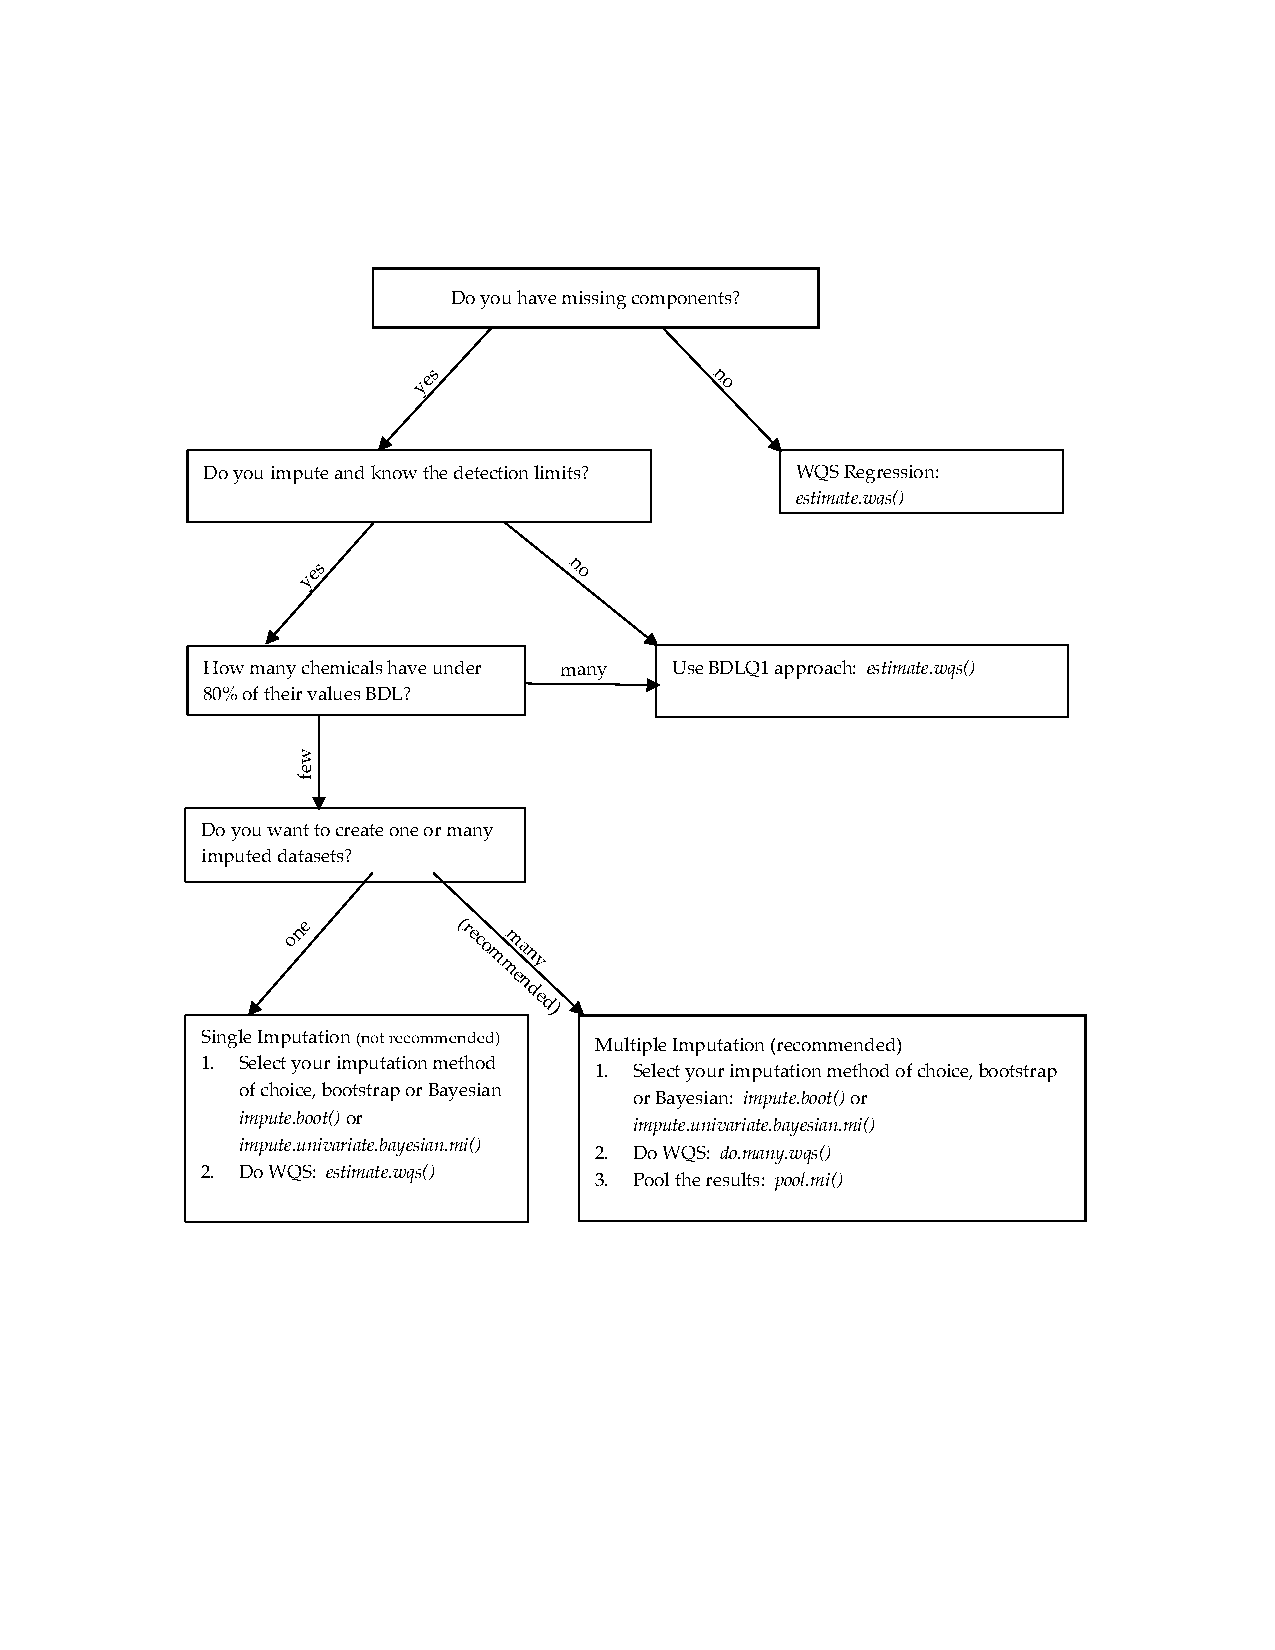
\includegraphics[width=1\linewidth]{figure-word/decision_tree.pdf} 

}

\caption{\label{fig::decide} A decision tree to help researchers in using the miWQS package. The package is flexible and can meet a wide range of needs.}\label{fig:fig.decide}
\end{figure}


\hypertarget{computational-details}{%
\section{Computational details}\label{computational-details}}

The functions in \pkg{miWQS} package relied upon code developed in other
packages on CRAN. The steps in the \code{estimate.wqs()} function also
relied upon other packages: the \code{solnp()} function in
\CRANpkg{Rsolnp} package \citep{ghalanosRsolnpGeneralNonLinear2015}, the
\code{glm2()} function in \CRANpkg{glm2} package
\citep[pg.~2]{marschnerGlm2FittingGeneralized2011}, the
\code{list.merge()} function in \CRANpkg{rlist} package
\citep{renRlistToolboxNonTabular2016}, the \code{format.pval()} in
\CRANpkg{Hmisc} package \citep{harrellHmiscHarrellMiscellaneous2020},
the \code{gather()} function from \CRANpkg{tidyr} package
\citep{wickhamTidyrEasilyTidy2020}, and the \CRANpkg{ggplot2} package
\citep{wickhamGgplot2ElegantGraphics2016}. The \code{impute.Lubin()}
function used the \CRANpkg{survival} package
\citep{therneauPackageSurvivalAnalysis2015}. The
\code{impute.univariate.bayesian.mi()} function used: the
\code{rinvgamma()} function in the \CRANpkg{invgamma} package
\citep{kahleInvgammaInverseGamma2017}, the \code{rtruncnorm()} function
in \CRANpkg{truncnorm} package
\citep{mersmannTruncnormTruncatedNormal2020}, the \code{possibly()}
function in the \CRANpkg{purrr} package
\citep{henryPurrrFunctionalProgramming2020a} and the \pkg{coda} package
\citep{plummerCODAConvergenceDiagnosis2006}. Additionally, the
\code{ggcorr()} function in the \CRANpkg{GGally} produced the heat map
in Figure \ref{fig::dataCorr}
\citep{schloerkeGGallyExtensionGgplot22020}.

This vignette is successfully processed using the following.

\begin{Schunk}
\begin{Soutput}
 -- Session info ---------------------------------------------------
\end{Soutput}
\begin{Soutput}
 setting  value                       
 version  R version 4.0.2 (2020-06-22)
 os       macOS  10.16                
 system   x86_64, darwin17.0          
 ui       X11                         
 language (EN)                        
 collate  en_US.UTF-8                 
 ctype    en_US.UTF-8                 
 tz       America/New_York            
 date     2021-01-20                  
\end{Soutput}
\begin{Soutput}
--  Packages -------------------------------------------------------
\end{Soutput}
\begin{Soutput}
 package   * version date       lib source                                 
 coda        0.19-4  2020-09-30 [1] CRAN (R 4.0.2)                         
 GGally    * 2.0.0   2020-06-06 [1] CRAN (R 4.0.2)                         
 ggplot2   * 3.3.3   2020-12-30 [1] CRAN (R 4.0.2)                         
 glm2        1.2.1   2018-08-11 [1] CRAN (R 4.0.2)                         
 gWQS        3.0.0   2020-06-23 [1] CRAN (R 4.0.2)                         
 Hmisc       4.4-2   2020-11-29 [1] CRAN (R 4.0.2)                         
 invgamma    1.1     2017-05-07 [1] CRAN (R 4.0.2)                         
 knitr     * 1.30    2020-09-22 [1] CRAN (R 4.0.2)                         
 mi          1.0     2015-04-16 [1] CRAN (R 4.0.2)                         
 mice        3.10.0  2020-07-13 [1] CRAN (R 4.0.2)                         
 miWQS     * 0.4.0   2020-07-27 [1] local                                  
 norm        1.0-9.5 2013-02-28 [1] CRAN (R 4.0.2)                         
 purrr       0.3.4   2020-04-17 [1] CRAN (R 4.0.2)                         
 rlist       0.4.6.1 2016-04-04 [1] CRAN (R 4.0.2)                         
 rmarkdown   2.3     2020-06-18 [1] CRAN (R 4.0.2)                         
 Rsolnp      1.16    2015-12-28 [1] CRAN (R 4.0.2)                         
 rticles     0.16.1  2020-09-22 [1] Github (rstudio/rticles@b0bbbc0)       
 survival    3.1-12  2020-04-10 [1] CRAN (                                 
 tidyr       1.1.2   2020-08-27 [1] CRAN (R 4.0.2)                         
 tinytex     0.26    2020-09-22 [1] CRAN (R 4.0.2)                         
 truncnorm   1.0-8   2020-07-27 [1] Github (olafmersmann/truncnorm@eea186e)
 wqs         0.0.1   2015-10-05 [1] CRAN (R 4.0.2)                         
 yaml        2.2.1   2020-02-01 [1] CRAN (R 4.0.2)                         

[1] /Library/Frameworks/R.framework/Versions/4.0/Resources/library
\end{Soutput}
\end{Schunk}

\hypertarget{acknowledgments}{%
\section{Acknowledgments}\label{acknowledgments}}

We like to thank Keith W. Zirkle and Anny-Claude Joseph for their
editorial comments on this vignette. Additionally, we thank the
anonymous reviewers of \emph{The R Journal} who have improved this
vignette. Lastly, we appreciate Yihui Xie's work in creating the
\CRANpkg{rticles} package that enabled us to write this vignette from
the Rmarkdown environment \citep{xieRticlesArticleFormats2020}.

\hypertarget{abbreviations}{%
\section{Abbreviations}\label{abbreviations}}

\begin{itemize}
\tightlist
\item
  AIC: Akaike information criterion
\item
  BDL: below the detection limit
\item
  BDLQ1: placing the BDL values into the first quantile
\item
  BMI: body mass index
\item
  CRAN: the comprehensive R archive network
\item
  DL: detection limit
\item
  GWAS: genomic wide association study
\item
  MCMC: Markov chain Monte Carlo
\item
  MI: multiple imputation
\item
  MI-WQS: multiple Imputation in connection with the weighted quantile
  sum regression
\item
  SES: socioeconomic status
\item
  SNPs: single nucleotide polymorphisms
\item
  WQS: weighted quantile sum
\end{itemize}

Notation: + \emph{n} sample size + \emph{c} number of chemicals +
\emph{K} number of imputations

\hypertarget{appendix}{%
\section{Appendix}\label{appendix}}

\hypertarget{deciding-whether-the-overall-mixture-effect-is-positively-or-negatively-related-to-the-outcome-in-wqs-regression}{%
\subsection{Deciding whether the overall mixture effect is positively or
negatively related to the outcome in WQS
regression}\label{deciding-whether-the-overall-mixture-effect-is-positively-or-negatively-related-to-the-outcome-in-wqs-regression}}

A researcher must decide whether the overall mixture effect,
\(\beta_1\), is positively or negatively related to the outcome in WQS
regression. One way is to perform a series of individual chemical
regressions and look at the sign of the regression coefficients. This is
performed via the \code{analyze.individually()} function. In each
regression, the outcome \(y\) is regressed on the log of each chemical
\(\boldsymbol{X}\) and any covariates \(\boldsymbol{Z}\) using the
\pkg{glm2} package \citep{marschnerGlm2FittingGeneralized2011}. Any
missing values are ignored. The arguments in
\code{analyze.individually()} are the same as the arguments specified in
\code{estimate.wqs()}. In \code{simdata87}, our outcome is element
\code{y.scenario}, the chemical mixture is \texttt{X.true}, the
covariates are contained in \code{Z.sim}. As the outcome in
\code{simdata87} is binary, we assign \code{"binomial"} to the
\code{family} argument. The \code{analyze.individually()} function
returns a data frame that consists of: the name of the chemical, the
individual chemical effect estimate and its standard error, and an
assessment of the WQS model fit using the Akaike Information Criterion
(AIC).

\begin{Schunk}
\begin{Sinput}
> analyze.individually(
+   y = simdata87$y.scenario, X = simdata87$X.true,
+   Z = simdata87$Z.sim, family = "binomial"
+ )
\end{Sinput}
\begin{Soutput}
       Chemical.Name Estimate Std.Error      AIC
1    alpha-chlordane    0.128     0.018 1315.527
2           dieldrin    0.176     0.033 1339.606
3    gamma-chlordane    1.310     0.192 1319.118
4            lindane    0.817     0.139 1332.276
5       methoxychlor    1.056     0.150 1315.461
6                dde    0.169     0.025 1319.293
7                ddt    0.176     0.086 1365.064
8  pentachlorophenol    0.245     0.081 1360.018
9            pcb_105   -0.026     0.051 1368.984
10           pcb_118    0.332     0.072 1347.162
11           pcb_138    0.356     0.056 1325.112
12           pcb_153    0.308     0.046 1321.903
13           pcb_170    0.404     0.087 1346.696
14           pcb_180    0.311     0.059 1339.602
\end{Soutput}
\end{Schunk}

The sign of the estimates indicates whether the overall mixture effect
should be positive or negative. As most of the estimates are positive
here, we will assume that the overall mixture is positively related to
the outcome. Then, we can set the \code{b1.pos} argument in
\code{estimate.wqs()} to be \code{TRUE}. In terms of model fit, the
complete-data mixture WQS model in \protect\hyperlink{Example-1}{Example
1} with an AIC of 660 fits the data better than any individual chemical
model (see the AIC's above).

\bibliography{hargarten-wheeler.bib}


\address{%
Paul M. Hargarten\\
Virginia Commonwealth University\\%
One Capitol Square\\ 830 East Main Street Seventh Floor\\ Richmond, Virginia 23219\\
%
%
%
\\\href{mailto:hargartenp@vcu.edu}{\nolinkurl{hargartenp@vcu.edu}}
}

\address{%
David C. Wheeler\\
Virginia Commonwealth University\\%
One Capitol Square\\ 830 East Main Street Seventh Floor\\ Richmond, Virginia 23219\\
%
%
%
\\\href{mailto:david.wheeler@vcuhealth.org}{\nolinkurl{david.wheeler@vcuhealth.org}}
}

